\documentclass[twoside]{report}
\usepackage[utf8]{inputenc}
%\usepackage[english]{babel}
\usepackage{amsthm}
\usepackage{tkz-fct} 
\usepackage{thmtools}
\usepackage[margin=1in]{geometry}
\usepackage{amsmath,amssymb}
\usepackage{multicol}
\usepackage{graphicx}
\usepackage{tikz}
\usepackage{listings}
\usetikzlibrary{positioning} 
\usetikzlibrary{calc,patterns,angles,quotes}
\usetikzlibrary{calc,arrows, arrows.meta}
\tikzset{
  arrow/.pic={\path[tips,every arrow/.try,->,>=#1] (0,0) -- +(.1pt,0);},
  pics/arrow/.default={triangle 90}
}
\usepackage{pgfplots}% also loads graphicx
\pgfplotsset{compat=1.11} %width=10cm,
\usetikzlibrary{backgrounds}
\usepackage{siunitx}
\sisetup{per-mode=fraction} %,fraction-function = \nicefrac}
\DeclareSIUnit{\gallon}{gal}
\usepackage{fancyhdr}
\usepackage{pst-node}
\psset{nodesep=2pt,linearc=2pt,arrows=->,linecolor=blue,arrowinset=0}
\def\lbl#1{\ncput*{\text{\tiny #1}}}
\usepackage{xcolor}
\usepackage{tcolorbox}
\usepackage{lmodern}
\usepackage{relsize}
\newcommand{\highlight}[1]{%
  \colorbox{red!50}{$\displaystyle#1$}}
\usepackage{url}
\usepackage{cancel}
\usepackage{mwe}
\usepackage{caption}
\usepackage{float}
\usepackage{setspace}
\usepackage{hyperref}
\usepackage{subcaption}
\usepackage{varwidth}
\usepackage{todonotes}
% set the arrows as stealth fighters (personal preference)
\tikzset{>=stealth}
\captionsetup[figure]{labelfont={bf},name={Figure},labelsep=period}

\declaretheoremstyle[
  spaceabove=6pt, spacebelow=6pt,
  headfont={\color{blue}\fontfamily{cmss}\selectfont\bfseries},
  notefont=\fontfamily{cmss}\selectfont\bfseries, notebraces={(}{)},
bodyfont=\fontfamily{cmss}\selectfont\itshape,
  postheadspace=1em,
]{mystyle}
\declaretheorem[style=mystyle,numbered=no]{definition}
\declaretheorem[style=mystyle,numbered=no]{lemma}

\declaretheoremstyle[
  spaceabove=6pt, spacebelow=6pt,
  headfont={\color{black} \fontfamily{cmss}\selectfont\bfseries},
  notefont=\fontfamily{cmss}\selectfont\bfseries, notebraces={(}{)},
bodyfont=\fontfamily{cmss}\selectfont,
  postheadspace=1em,
  qed=$\triangle$
]{mystyle2}
\declaretheorem[style=mystyle2,numbered=no]{remark}

\declaretheoremstyle[
  spaceabove=6pt, spacebelow=6pt,
  headfont={\color{orange} \fontfamily{cmss}\selectfont\bfseries},
  notefont=\fontfamily{cmss}\selectfont\bfseries, notebraces={(}{)},
bodyfont=\fontfamily{cmss}\selectfont,
  postheadspace=1em,
  qed=$\triangle$
]{mystyle3}
\declaretheorem[style=mystyle3,numbered=no]{example}

\declaretheoremstyle[
  spaceabove=6pt, spacebelow=6pt,
  headfont={\color{blue} \fontfamily{cmss}\selectfont\bfseries},
  notefont=\fontfamily{cmss}\selectfont\bfseries, notebraces={(}{)},
  bodyfont=\fontfamily{cmss}\selectfont\itshape,
  postheadspace=1em,
  qed=
]{mystyle4}
\declaretheorem[style=mystyle4,numbered=no]{law}

\declaretheoremstyle[
  spaceabove=6pt, spacebelow=6pt,
  headfont={\color{blue} \fontfamily{cmss}\selectfont\bfseries},
  notefont=\fontfamily{cmss}\selectfont\bfseries, notebraces={(}{)},
bodyfont=\fontfamily{cmss}\selectfont,
  postheadspace=1em,
  qed=
]{mystyle5}
\declaretheorem[style=mystyle5,numbered=no]{strategy}

\declaretheoremstyle[
  spaceabove=6pt, spacebelow=6pt,
  headfont={\color{blue} \fontfamily{cmss}\selectfont\bfseries},
  notefont=\fontfamily{cmss}\selectfont\bfseries, notebraces={(}{)},
bodyfont=\fontfamily{cmss}\selectfont\itshape,
  postheadspace=1em,
  qed=
]{mystyle6}
\declaretheorem[style=mystyle6,numbered=no]{theorem}


\renewcommand{\qedsymbol}{\rule{0.7em}{0.7em}}
\renewenvironment{proof}{{\bfseries \fontfamily{cmss} \scshape Proof:}}



\newcommand{\reporttitle}{##}
\newcommand{\reportauthor}{Kai Cooper\\Yacine Trad\\Yehao Liu\\ ZachHFT}
\newcommand{\reportsecondauthor}{}
\newcommand{\reportthirdauthor}{}
\newcommand{\reportfourthauthor}{}
\newcommand{\reportfifthauthor}{}
\newcommand{\supervisor}{Dr. Mehdi Gholam \\ Celia Garcia Pareja}

\date{June 2021}

\renewcommand{\chaptername}{Part}
\newcommand{\lap}{\nabla^2}
\newcommand{\dif}[1]{\text{d}#1}

\newcommand{\code}{\texttt}
\renewcommand{\floatpagefraction}{.8}

\definecolor{fcolor}{RGB}{0,255,255}

\usepackage[numbers]{natbib}

\begin{document}
\begin{spacing}{1}
\input{SCV_Crypto_Report(s)/titlepage}
\fontfamily{cmss}\selectfont
\tableofcontents




\chapter{Introduction}

\section{Background and scope}
Let's begin by presenting a general overview, during which we'll go through the key-terms needed to understand this project.

When faced with a given cryptocurrency, what we see on a price chart is the value of a single \textbf{token}.
The value of a token is equal to the market cap (total value of the network noted MC) of a currency divided by the total circulating supply (number of tokens noted CS).
Bitcoin has a circulating supply of 19 million tokens but a total supply of 21 million tokens. The difference between the circulating supply and the total supply is the amount still available to be mined, and indicates future inflation. 
$$\text{Token}_\text{BTC}=\frac{\text{MC}}{\text{CS}}$$
\begin{figure}[!htbp]
    \centering
    \includegraphics[scale = 0.7]{TestPlots/BTC_overview.png}
    \caption{The price chart of Bitcoin from 2017 to 2021}
    \label{BTC overall}
\end{figure}

Just by looking at the chart in Figure \ref{BTC overall}, one can realise how volatile bitcoin has been and this particularity is shared by many other cryptocurrencies.\\
Bitcoin went from $10\text{K}\$$ in September 2020 to over $60\text{K}\$$ in April 2021, but also lost half of it's value from April to July 2021.
One can say without doubt that the prices are on a roller coaster, everyone wants to experience the upward trends however the downfalls are extremely scary.\\

Of course, not all cryptos follow the same trends some might be rising while others are crashing, and the goal of crypto-trading is to ride the right wave at the right time, and jump off the ship before it sinks. That is why we will be dealing with crypto pairs which are explained further.\\
The prices fluctuate according to many variables such as news, regulations, announcements, general sentiment etc... Of course risk is involved and that's why the best way to navigate these dangerous waters is to have a set plan and the right logic to follow.







\section{Aim}

The goal of this project is to proceed to the analysis of an optimal trading (buy-and-sell) strategy for the market of Cryptocurrencies. In particular, we will investigate 4 range of strategies, namely, a first general Exploratory Data Analysis which shall lead us to discover some general historical trends over the days and months of trading (e.g. Thursday is generally a bad day to trade Bitcoin with a negative log-return overall). Secondly, we will investigate how social networks influences cryptocurrencies prices, we will propose buy-and-sell strategies accordingly, and shall backtest the latter. Later on in the project we shall proceed to analysis of cryptocurrencies interactions, cycles, and trends forecasting. We wish to pick the top trending cryptocurrencies right before they actually become top-trending cryptocurrencies. Eventually we shall conclude this project with the analysis of extremes. \\


Before starting our analysis, the reader should know that, unlike stock markets, for which financial data are extremely onerous, cryptocurrencies data are far less expensive and far more accessible. In particular, we use Binance's (a major cryptocurrency exchange platform) API to extract the historical trading prices of every exchange pair on its platform. It's API allows us to obtain the historical prices over 1 day, 1 hour, and even 1 minute period. We shall obtain open, high, low, close (OHLC) prices for the according period. The trading volume is also provided. We provide further details regarding these data in the next section.\\



If you do not want to get your hands dirty (which is understandable) navigating through the code to download the data, simply download a subset of the historical data we use at this link : \url{https://drive.switch.ch/index.php/s/URDxQbEv8LqSkB2}




\section{Data}
\subsection{Data extraction and processing}


Note that we have never encountered any NA values or other seemingly out-of-place values that would need to be rejected. Indeed, so called 'out-of-place values' or any other outliers kind of value are strong indicators which require further investigations and may be relevant to dedicated algorithmic trading strategies. We absolutely do not want to remove them as we may be tempted to do in some other contexts in data science.\\

Discrepancies in the timestamp of our data : Missing time periods. Every once in a while there is a major crash in cryptocurrencies market (i.e. prices dropping significantly). This leads to a massive amount of people trying to connect to the cryptocurrencies exchange platforms to try to sell (or buy) some cryptocurrencies.This often results in the exchange becoming unavailable, their server not being able to handle so many connections attempts at once. This explains the missing data in historical cryptocurrencies prices data (It can be for a couple of minutes up to a couple of hours). We therefore compute 'time\_diff\_in\_days' and 'time\_diff\_in\_min' to spot any such discrepancies in the timestamp. For example, in a 1-hour dataset we expect that time difference between line i and line i-1 to be 60 min. If it appears to be 57 minutes, we know there was a crash that occured and therefore can decide our backtesting programme to not consider (i.e. to pause) this very particular time period. It is a useful method to rigoursly proceed to backtesting algorithm. \\



It is important to note that sometimes the dataset obtained via the extraction in Python can have missing rows of data, i.e. a time series with some missing dates/times depending on the resolution of the data set. As our analyses will be making decisions at every time step in the relevant dataset, this is inconvenient. One way to circumvent this is to \textbf{impute} the time series, and there are software packages available to do this. For example, in section \ref{reddit} on Reddit networks, an R package called \code{imputeTS} is used to do this, with the function \code{na\_kalman} which replaces \code{NA} values in the dataset using nearby values by Kalman Smoothing []. This method is one of the most recommended in the package [],

\begin{figure}[H]
    \centering
    \includegraphics[width=\linewidth]{Reddit_Analysis/Price_Data_Extraction/Data/Binance_OHLC/imputed_gg_1m.png}
    \caption{Imputed values of time series. The graph is generated automatically with the function \code{ggplot\_na\_imputations} in the \code{imputeTS} package.}
    \label{fig:imputations}
\end{figure}


Going further, once an analysis is performed on a dedicated dataset (e.g. 1 hour BTC/USDT historical data), the same statistical analysis can be performed over any dataset (e.g. 1 minute ETH/CHF historical data), since the data structure (i.e. the columns, open, high, low, close) is the same. We shall do so later on in the project.



\subsection{Data transformation}

The goal of this project is to proceed to the analysis of an optimal trading (buy-and-sell) strategy for the market of Cryptocurrencies. Our analysis will be made on cryptocurrency pairs.\\
These pairs allow us to compare costs between different cryptocurrencies. They are helpful for illustrating the relative worth of coins. For example,the question how much Bitcoin (BTC) equals in Ethereum (ETH) will be answered by the value of the pair BTC/ETH.
In this report we are dealing with the BTC/USDT pair. USDT stands for Tether which is a stable coin in which each token is backed by a U.S Dollar.\\
The price of a token depends on the market cap of the currency and how many tokens are issued. And since there are hundreds of cryptocurrencies dealing with their prices can become very cumbersome and lack clarity. For that very reason, we have chosen to deal in our analysis with log-returns.
Indeed, the price of a currency is not what is of interest to us but rather it's evolution. By studying prices we would be confronted with values that don't have an intrinsic meaning, However with log returns we will have an idea of the evolution in percentages, which is way more useful. To sum it up, this allows measuring a lot of variables in a comparable metric, thus enabling evaluation of analytic relationships amongst two or more variables despite originating from price series of unequal values. \\
Concretely, if we are doing our study on a currency at time $i$ which is valued at price $p_i$. The log-return for the period $t$ is:
$$\log\left(\frac{p_i}{p_{i-t}}\right)$$\\

Another important property is the additivity of the log-return. If our price at $t_1$ is $p_1$, it changes to $p_2$ at $t_2$ and move to $p_3$ at $t_3$. The log return from $t_1 $ to $t_2$ is $\log (p_2) - \log (p_1)$, the log return from $t_2 $ to $t_3$ is $\log (p_3) - \log (p_2)$. Therefore, it is clear that the log return from $t_1 $ to $t_3$ is $\log (p_3) - \log (p_1)$. This can be calculated easily. However, if we use simple return, the return should be $p_3/p_1$ instead of $p_3/p_2 + p_2/p_1$. Hence, log-return is easier to apply to real data.

 An interesting observation one can make when plotting the log-returns is that they are supposed to be normally distributed.
 
 
 \section{Exploratory data analysis}
Exploratory data analysis (EDA) is used in data analysis to analyze and investigate data sets and summarize their main characteristics. It helps determine how best to manipulate data sources to get the answers you need, making it easier to discover patterns, spot anomalies, test a hypothesis, or check assumptions.

EDA is primarily used to see what data can reveal beyond the formal modeling or hypothesis testing task and provides a provides a better understanding of data set variables and the relationships between them. It can also help determine if the statistical techniques you are considering for data analysis are appropriate. Originally developed by American mathematician John Tukey in the 1970s, EDA techniques continue to be a widely used method in the data discovery process today.

The main purpose of EDA is to help look at data before making any assumptions. It can help identify obvious errors, as well as better understand patterns within the data, detect outliers or anomalous events, find interesting relations among the variables.



\subsection{Distribution of prices and returns}




Figure (\ref{log return box}) shows the box plot of log-return of BTC. As can be seen from the graph, the mean value of log-return changing is around 0. with the first and third quantile around -0.02 and 0.02. It is worth mentioning that there are lots of outliers. This means the price change drastically for some certain days.



Figure \ref{7day rolling volume} is about 7 days rolling average of the volume. As the average volume is different within a week (In the weekday, there are more trades than in the weekend), we calculate the average volume of 7days to smooth the plot. From this figure, we see that the volume oscillate during our examining period. The volume sometime change drastically for a certain day. However, with the existence of up and down signals, we see there is a trend of volume increasing from the beginning of 2017-07 to 2021-07.


\begin{figure}[!htbp]
\centering
\begin{subfigure}{.5\textwidth}
    \centering
    \includegraphics[width=.9\linewidth]{Images/Box Plot of Return.png}
    \caption{Box plot of log-return}
    \label{log return box}
\end{subfigure}%
\begin{subfigure}{.5\textwidth}
    \centering
    \includegraphics[width=.9\linewidth]{Images/Volume Rolling Average.png}
    \caption{7 day rolling average of the volume}
    \label{7day rolling volume}
\end{subfigure}
\caption{(a) The box plot of log-return of BTC in the given period. (b) The line plot of the rolling average of the volume}
\label{fig:test}
\end{figure}

\subsection{Mean hourly BTC/USDT log-return by day, by week, and by month}

In the following we show historical average hourly log-return based on the trading day, the trading week, or the trading month.
\\ \\
We can notice that historically, Thursday is a bad trading day, and if historical trends are any indication of future trends, we may want to consider avoiding trading on this particular day.
\\ \\
Similarly, we see that the months of March and September are historically quite bad months to trade and we may want (assuming this trend will repeat in the future) selling our BTC assets in the beginning of these months and buying back at the end of these months.
\\ \\
We display the charts below.
\begin{figure}[!htbp]
    \centering
    \includegraphics[scale = 0.5]{Images/Average hourly log-return for BTCUSDT per day.png}
    \caption{Average hourly log-return for BTCUSDT per day}
    \label{Average hourly log-return for BTCUSDT per day}
\end{figure}

\begin{figure}[!htbp]
    \centering
    \includegraphics[scale = 0.5]{Images/Average hourly log-return for BTCUSDT per week number.png}
    \caption{Average hourly log-return for BTCUSDT per week number}
    \label{Average hourly log-return for BTCUSDT per week number}
\end{figure}

\begin{figure}[!htbp]
    \centering
    \includegraphics[scale = 0.5]{Images/Average hourly log-return for BTCUSDT per month.png}
    \caption{Average hourly log-return for BTCUSDT per month}
    \label{Average hourly log-return for BTCUSDT per month}
\end{figure}


\subsection{Analysis of extremes}

\begin{figure}[!htbp]
    \centering
    \includegraphics[width=\linewidth, scale=0.8]{Extremal Modelling/distplots_sans_outliers.png}
    \caption{Distribution of log returns having eliminated outliers and a QQ plot of the data against a standard normal random variable. Clearly the data is still heavily tailed.}
    \label{fig:distplots_sans_outliers}
\end{figure}


In finance, the question of extreme values is indubitably an important one. For example: stock market crashes, interest rates ad  insurance pricing based on life expectancy are all fields in which it would be necessary to consider rare events. The analysis of cryptocurrency trajectories is no different, indeed, sudden but large deviations in the trajectory of cryptocurrency prices would certainly be of interest to a trader. 

In light of this, it is not unnatural to ask the corresponding statistical question in the context of extremes. In Figure \ref{fig:distplots_sans_outliers}, we can see that the distribution of log returns for our data set admits very heavy tails. In this dataset there are many statistically anomalous results which skew the data, but even upon their removal, the data remain strongly skewed, see Figure \ref{fig:distplots_sans_outliers}, the data still exhibit this skewed behaviour. This sparks interest in using extreme value theory to aid our understanding of this behaviour.\\

If we observe a trajectory of prices $p_t$, for $t$ an index of time (e.g. prices per minute or hour, etc.), by assuming they come from a random sample, we can aim to fit their scaled extreme, either maximum or minimum, to a distribution of the following type \[
G(x; \eta, \tau, \xi) = \begin{cases}
\exp\left[-\left\{1+\xi(x-\eta)/\tau\right\}_+\right], & \xi \ne 0\\
\exp\left[-\exp\left\{-(x-\eta)/\tau\right\}\right], & \xi = 0,
\end{cases}
\]
where $\eta, \tau$ and $\xi$ are location, shape and scale parameters respectively. Studying maxima in this way is called the \textbf{block maxima approach}, since one groups data and considers fitting the distribution to the maxima across all groups, for example: maximum price over one day, where the prices are indexed by hours.

The goal, then, would be to fit this model to our data, i.e. by finding the unknown parameters. To this end, we have available to use the R packages $\code{evd}$ and $\code{ismev}$ which give useful functions for extremal modelling and makes plotting diagnostics straightforward. We will demonstrate their capabilities in later sections. 





\chapter{Social media's influence on cryptocurrency prices}

Unlike the traditional stock market, cryptocurrencies are traded without many regulations and are accessible to essentially anyone with an internet connection. Therefore it is not surprising that cryptocurrencies are perhaps more sensitive to human behaviour than traditional stocks; including a much more chaotic response to sudden trends and attitudes of these traders. This is indubitably heavily impacted by social media. We aim in this chapter to leverage this observation to generate winning strategies for trading on the market. 

\section{Youtube trends}

Youtube is the most dominant streaming platform worldwide. Many youtube channels are focused solely on cryptocurrencies and they do, sometimes, impact small market cap cryptocurrencies. In general, low market cap cryptocurrencies (below 10M USD) historical prices and data are hard to access and require APIs from numerous cryptocurrency exchanges each. Therefore, we will here confine ourselves to a general trend analysis of popular crypto Youtube channels.\\

First we seek to figure out the search trends of Youtube, using Pytrends, an API for Google Trends, which allows us to retrieve the trending on Google search engines, including Youtube. We get the most trending queries on Youtube for the word 'Cryptocurrency'. From these we see four popular cryptocurrencies channel stand out, namely: Bitboy crypto, Banter crypto, Jrny crypto, and Crypto zombie.\\

We then seek to observe the interest over time of each of these channels, as seen in Figure \ref{youtube_channel_crypto_trends}.

\begin{figure}[!htbp]
    \centering
    \includegraphics[scale = 0.5]{Images/youtube_channel_crypto_trends.png}
    \caption{Bitboy Crypto charges 60k USD to publish a video on upcoming cryptocurrencies, as per his notoriety.}
    \label{youtube_channel_crypto_trends}
\end{figure}


Eventually we seek to observe the interest by region of one particular channel, Bitboy Crypto, a famous youtuber known to be influential in the sphere. If you are interested in map visualization, we use Choropleth map provided by Folium python package. We can see his viewership is mostly in the anglosphere, as we shall expect.

\begin{figure}[!htbp]
    \centering
    \includegraphics[scale = 0.5]{Images/countries_rank_bitboy_crypto_youtube.png}
    \caption{Bitboy Crypto is unsuprisingly most trending in anglophone countries.}
    \label{countries_rank_bitboy_crypto_youtube}
\end{figure}

\begin{figure}[!htbp]
    \centering
    \includegraphics[scale = 0.4]{Images/countries_map_2.png}
    \caption{Map of the countries most trending for the Youtube channel Bitboy Crypto}
    \label{countries_map_2}
\end{figure}


\section{Twitter}
Twitter is an American microblogging and social networking service on which users post and interact with messages known as "tweets". Users can post, like, and share (or retweet) tweets. Millions of people from a wide variety of positions and backgrounds react and share their opinions on the platform. This includes people of great significance  and influence within society, for example the former president of the US, Donald Trump, used Twitter extensively to communicate with the American citizens during his mandate.

One finds that some individuals are very aware of the impact they have on social media and often use their influence unreservedly. Elon Musk, a very well-known serial entrepreneur and founder of Tesla, who is also the richest man on the planet, has been heavily criticized for his influence on a few cryptocurrency stocks. He has embraced his role and was proclamed the Doge Father by the crypto community in reference to the cryptocurrency Dogecoin. He has been creating immense moves (both up and down) of price charts with his tweets.

\subsection{Twitter strategy}
Elon Musk's tweets unquestionably have great power. To create great profit inducing trading strategies it serves to try and quantify the power influencers like Elon Musk possess. In this section we will explore a simple trading strategy applied to BTCUSDT and DOGEUSDT currency pairs: \begin{strategy}[Elon Musk]
Buy $1000\text{\$}$ whenever Elon musk tweets about a given cryptocurrency and hold this position for 24 hours. Once the 24 hour period has ended, sell the stock.
\end{strategy}\label{strat:musk} 
We will visualise the effectiveness of this strategy through the \textbf{profit and loss} (PnL) generated by this strategy. If our portfolio (number and type of quantities traded) has value $V_t$ for $t$ an index of time, then the sequence $(V_t)_{t=0}^T$ for some end-time $T$ is called the profit and loss of the portfolio through time.

Users interact with Twitter through browser or mobile front-end software, however in order to collect their data from that platform computationally one has to do it via Twitter's APIs in a similar way to what we did to get the data from Binance.
We have used the python library \code{snscrape.modules.twitter} to collect the data we needed. We then updated the buy signal accordingly. We have scraped Elon Musk's tweets in search of occurrences of the character strings 'BTC', 'bitcoin', 'dogecoin' or 'DOGE' to create the datasets dealing with bitcoin and dogecoin respectively. To do that we have used the function \code{sntwitter.TwitterSearchScraper}. Here are the results. \\

\begin{figure}[!htbp]
    \centering
    \includegraphics[scale = 0.5]{TestPlots/plot-BTC-pnl.png}
    \caption{Although This strategy leads to a 20\% increase of the value of our portfolio for Bitcoin overall. We notice the presence of both a big up-trends and massive drops.}
    \label{}
\end{figure}

\begin{figure}[!htbp]
    \centering
    \includegraphics[scale = 0.5]{TestPlots/plot-DOGE-pnl.png}
    \caption{The strategy looks better for Doge and we can see a 100\% increase of the initial investment.}
    \label{}
\end{figure}

 Tweets have a noticeable effect on the price of a currency, however, a tweet can negatively impact the price and suggests that one should pay attention to what is said in a tweet.\\
For instance the huge up-trend after the $10^{th}$ entry point corresponds to a tweet in which he said "You can now buy a Tesla with Bitcoin" [24/03/2021]. We can infer that, this short sentence gave people a lot of hope and showed the interest of a massive company towards the cryptocurrency. The uptrend continued but then he talked about the risks and limitations of Bitcoin and said ``Bitcoin is actually highly centralized, with supermajority controlled by handful of big mining (aka hashing) companies. A single coal mine in Xinjiang flooded, almost killing miners, and Bitcoin hash rate dropped 35\%. Sound “decentralized” to you?" %\cite{Elon}[16/05/2021]. 
From this we can infer that bitcoin traders lost confidence in the cryptocurrency, to use the crypto slang it spread FUD (fear uncertainty and doubt), and that caused a massive drop of the price.\\
Knowing that a single person had so much power and could influence the prices easily in either way scared investors and Elon Musk received a lot of criticism and was accused of purposely affecting the markets to push his company's agenda. This criticism has led to a noticed dampening effect of his tweets \cite{ElonCriticism} \\
Following this logic, it seemed natural to try to get a sense of how optimistic a tweet was before deciding whether or not to buy.\\
For that very reason we have chosen to use the python library \code{textblob} \cite{loria2018textblob} for processing textual data and proceed to the sentiment analysis of the tweets. The function \code{sentiment.polarity} gave a score in $ [-1,1]$ indicating how positive a text is using averaging methods. For instance : \[\code{sentiment.polarity}(``\text{good}")=0.7\;\;\;\:\:\code{sentiment.polarity}(``\text{bad}")=-0.7.\]
\begin{strategy}[Adding Sentiment]
We have added to the previous strategy the condition that the tweet had to have a sentiment score greater or equal to $0.2$ for us to buy.\end{strategy}\label{strat:sent} 
\begin{figure}[!htbp]
    \centering
    \includegraphics[scale = 0.5]{TestPlots/plot_sentiment_btc.png}
    \caption{The sentiment condition has missed on great upward motions as well as drops, the portfolio value still raised but only by 6\%. Which is not significant at all, especially for crypto stocks.}
    \label{}
\end{figure}
\begin{figure}[!htbp]
    \centering
    \includegraphics[scale = 0.5]{TestPlots/Doge_sentiment_plot.png}
    \caption{The strategy is clearly not efficient for doge. We lose on our position most of the time. }
    \label{}
\end{figure}

This  reduced the number of entry points by more than a half but missed out on great opportunities while doing so. That is probably because neutral sentences containing crucial information can be misinterpreted by the sentiment function. Indeed the sentence "you can buy tesla with bitcoin" has a score of $0$, While the sentence "bitcoin consumes too much energy" has a score of $0.2$.

Of course this is also because our person of interest, Elon Musk, is not trying to energize the public but just making an announcement. In conclusion trying to gauge the sentiment of his tweets wasn't the best approach, and resulted in a loss of capital.

Sentiment analysis is an efficient technique and should be used at a bigger scale when analyzing an important amount of tweets coming from different people, using it on a single person could lead to errors due to the personality of the source.





\section{Medium}\label{sec:medium}
Medium is an American online publishing platform developed by Evan Williams and launched in August 2012. The platform gives its members the ability to read and participate in social journalism, having a hybrid collection of amateur and professional people and publications. The site is regularly regarded as a blog host \cite{streitfeld2017internet}.




As we know, many cryptocurrencies are run by companies or individuals. They maintain the currency they create, and they use social media to promote their cryptocurrency. Medium, as a famous and influential social media platform, is often used to promote the cryptocurrency they create. One idea we came about is that there may have some relationships between the medium and price changing of their cryptocurrency. In this section, we aim to develop strategies using the information from their medium blog. As an example, we focus on a certain cryptocurrency called Kyber (KNC). Though there are differences between each cryptocurrency, the analysis and the strategies can be applied to other cryptocurrencies as well. 



\subsection{Data Preprocessing}
In this section, we explain how we access the data from the medium and the changes of cryptocurrency price. For the medium publications, we use webscraping techniques via some python libraries (\code{BeautifulSoup4 , request} and \code{selenium}). At first, we use \code{request} to acquire the source code of the website from \url{https://medium.com/@kyberteam}. This allows us to access the information via the python.  With the help of library \code{selenium}, we are able to acquire the full information of the source code. After that, we use functions in the library \code{BeautifulSoup4} to parse the whole source code. By doing so, we can deal with this HTML information much easier with Python. With the \code{find\_all} function, we can find all information that interests us in each article. In our case, we think the update time of the article and the title of the article might be helpful for developing strategies. Therefore, using techniques we just introduced, we have a dataframe that contains the update time (denoted as \code{date}) and title for all of the medium articles (denoted as \code{title}) from Kyber.

When looking into details, we found that they do not update their medium everyday. We guess updating an article or not is a good signal in developing strategies. So we make a new feature called \code{signal}. It is a binary variable, and the entry is given value 1 if Kyber posted on that day at medium and 0 otherwise.  For the \code{title}, we want to apply sentiment analysis used in Twitter and keyword checking (To see if it contain certain keyword like 'announcement') at first. However, as a big company based in Asia, Kyber published a large amount of articles that not in English. As a result, it is not easy to do the analysis based on these different languages.  




Another work is about the preprocessing of the price changing data. To achieve this goal, we us an API from Binance to access to the cryptocurrency price. Binance is a cryptocurrency exchange which is currently the largest exchange in the world in terms of daily trading volume of cryptocurrencies. With the help of Binance API, we are able to extract the details for price changing of Kyber and analysize it with Python. We put these details into another dataframe, and merge it with the dataframe with medium information. After choosing relevant information, we have some features that are listed in the Table \ref{tab:feature}. 

As the Kyber begun to trade on Binance since 2020-06-12, the data we select are between 2020-06-12 to 2021-11-16.


\begin{table}[!htp]
    \centering
    \begin{tabular}{|l|p{0.8\linewidth}|}
        \hline
        \code{date}  & Date of trading \\
        \code{high} & The highest price of the day\\
       \code{low}& The lowest price of the day\\
       \code{close} & The close price of the day\\
       \code{Open}& The open price of the day\\
         \code{signal} & Binary indicator vector of Kyber article posts indexed by day. An entry is given the value $1$ if Kyber posted on that day and $0$ otherwise.\\
         \code{opcl}  & The log difference between the open price and close price \code{$\log(close)-\log(open)$} \\
        \code{volume} & The amount of money traded at that day.\\ \hline
    \end{tabular}\vspace{2mm}
    \caption{Summary of the features from our final dataframe. On the left hand it is the feature name of data, while the right hand is the definition of them. The only feature that is obtained via the function of other features is \code{opcl}. This is an important feature for developing strategies }
    \label{tab:feature}
\end{table}


\subsection{Statistical Analysis}
We will investigate the strength of correlation between \code{opcl} and other features. If we find some strong correlations between \code{opcl} and some features, we can use that fact to inform a great trading price within a day. In order to do that, we use python to calculate the Pearson's correlation between them.   Unfortunately, we can't find any features that strong correlate with the \code{opcl}. As can be seen from figure (\ref{medium stats}), the correlations between all the features and \code{opcl} are small. The abosolute value of them are less than 0.4, which means there is no correlations or weak correlations. Therefore, we cannot use this correlation result directly to develop a new strategy.

\begin{figure}[!htbp]
    \centering
    \includegraphics{Images/Medium stats.png}
    \caption{The correlation between \code{clop} and features mentioned in the features table (\ref{tab:feature}). As can be seen, all of these correlations are less than 0.4. There are no direct correlation between these features, and we can't have a direct way to develop the strategy}
    \label{medium stats}
\end{figure}


\subsection{Medium Strategy }
From statistical analysis, we can't find a 



\begin{strategy}[Kyber Next Day]
If Kyber updates an article on date $t$, we spend all the money to buy the cryptocurrency on date $t$ with the open price and sell them all at the open price on date $t+1$.
\end{strategy}\label{strat:Kyber1}

\begin{strategy}[Kyber Same Day]
If Kyber updates an article at some time $t$, we spend all the money to buy the cryptocurrency at the open price on date $t$ and sell at the close price on date $t$.
\end{strategy}\label{strat:Kyber2} 

We compare the two strategies with a baseline, which is the simplest strategy: buy the cryptocurrency and do nothing. The value of our portfolio created this way is simply the price of the cryptocurrency over time. To perform the analysis, we assume that we have $1000$ dollars at the start of the strategy's implementation. Figure \ref{backtest medium} is the figure of price change of the two strategies and the baseline.

\begin{figure}[!h]
    \centering
    \includegraphics[scale =  0.65]{Images/medium backtesting.png}
    \caption{Back testing of two strategies mentioned above. All the money are in USD. It can be seen clearly that the two strategy outperform the baseline the majority of the time.}
    \label{backtest medium}
\end{figure}

Clearly, the naïve do nothing strategy is sub-optimal. We see that this strategies perform very well between day 80 to day 200, where the price of Kyber drops drastically. However, they couldn't escape the big crash on day 475, and the two strategies suffer a great loss during this time. In conclusion, these two simple strategies outperform the baseline, while the second strategy performs the best.

\section{Reddit}\label{reddit}
Reddit is the Internet's forum. It serves as a hub for discussion on just about anything you can think of. Naturally, therefore, cryptocurrency enthusiasts will discuss trends, advice and more in the many dedicated fora such as 'r/Cryptocurrecy' or 'r/Bitcoin'. For this reason, it is not hard to imagine that there are more prominent members of the community who feature across several fora and make frequent contributions to the community. Over time, these people may gain a reputation for some type of expertise. Such people, like in the Twitter section, we will call  \textbf{influencers}. 

But how can we identify such people? Reddit is largely anonymous, and many important members of the community aren't as easily identifiable as Elon Musk. Therefore, it is important to not treat this question subjectively, since that could lead to the omission of potentially important authors whose contributions to the network of crypto traders have been valued. Consequently, we make a superficial\footnote{due to time constraints} use of network science to locate these users. 

\subsection{Reddit as a social network}\label{sec:redditSN}

Reddit, by definition, is a social network. It connects human beings together through online interaction. Therefore it lends itself to being represented mathematically in this way. However, there are many ways to do this. To list some examples, one could form: a network of fora which share users; a network of users and those who comment on their posts or a network of fora and their users. Each of these cases present distinct sets of network elements: the first, a set of fora; the second, a set of users while the third is an interesting mélange of the two. 

To illustrate the sheer versatility of this approach, and introduce some of the ideas used in our analysis, we begin by forming several networks (or interchangeably, \textit{graphs}) based on subreddits and users centered at the \textbf{r/CryptoCurrency} subreddit. The data were accessed using the extensive \code{praw} library in Python, which is used for webscraping essentially all publicly visible Reddit data. 

Before we begin, let us define some terminology that will be used throughout this section. A \textit{subreddit} is a forum dedicated to a given topic; these terms will be used interchangeably. A user, author or \textit{redditor}, is someone who actively uses reddit by making \textit{submissions} or posting \textit{comments} on those submissions, where the former are posts that start a \underline{discussion} within a subreddit. In this section, we will often work with 'top' posts. These are posts that have been identified as popular or highly rated by Reddit users. If you're not already familiar, please visit the site (\url{www.reddit.com}) and have a look around, there are myriad topics there and indubitably one will catch your eye!\\ 

We will access a set of users who have posted in the r/CryptoCurrency subreddit across the top $500$ submissions in recent history. Their activity in the subreddit is shown in Figure \ref{fig:num_posts_r_crypto}. 

\begin{figure}
    \centering
    \includegraphics[width=0.8\linewidth]{Reddit_Analysis/Network_Analysis/num_posts_r_crypto.png}
    \caption{The number of posts an author makes in the r/CryptoCurrency subreddit. Notice that the names of the authors do not identify actual people, they are just online handles. This anonymity means that a truly objective approach need be taken to discover influential members of the community, before their impact is analysed.}
    \label{fig:num_posts_r_crypto}
\end{figure}

\begin{figure}
    \centering
    \includegraphics[width=0.8\linewidth]{Reddit_Analysis/Network_Analysis/other_subs_contributions.png}
    \caption{The other subreddits frequented by users of the r/CryptoCurrency subreddit have underlying themes. Notice that r/Bitcoin, r/ethtrader, and r/investing are some of the most discussed by users of r/CryptoCurrency.}
    \label{fig:other_subs_contributions}
\end{figure}

%\begin{figure}
 %   \centering
  %  \includegraphics[scale=.525]{Reddit_Analysis/Network_Analysis/Network Graph of Related Subreddits.png}
  %  \caption{Caption}
  %  \label{fig:my_label}
%\end{figure}


Our goal for the moment is exploratory and we will investigate several properties of the users and related subreddits of r/CryptoCurrency. In this context, what do we mean by related? Here, we will also identify the subreddits in which the top authors in r/CryptoCurrency are also active, see Figure \ref{fig:other_subs_contributions} for a vusualisation. It is no surprise that subreddits like r/Bitcoin and r/ethtrader appear, while we also see that r/memes is popular as it is a general, fun forum.

To analyse this structure more deeply, we create a network, $G$, connecting these authors and subreddits. To do this, we used the extensive \code{networkX} library in Python, which has extensive documentation describing all its capabilities. The network is formed in the following way: if redditor $r$ posts in subreddit $s$, then we connect $r$ and $s$ by a \textbf{link}, which we may denote $r \sim s$ (read as: $r$ is linked to $s$). We say that the \textbf{nodes} of this network are the elements connected via a link. One should notice that a network constructed in this way has a special property. It is possible to separate the set of nodes $V$ of $G$ into two disjoint groups or \textbf{categories} $R$ and $S$ where there exist no links between pairs of nodes where each node belongs to the same set: such networks are called \textbf{bipartite}.

The substructures of networks of this type are often of interest to analysts; indeed, bipartite networks admit two \textit{projections} which reveal the underlying structure. For example, we can form a network between subreddits, $s, s' \in S$, where $s \sim s'$ whenever there is an $r$ such that $r \sim s$ and $r\sim s'$. In words: if a redditor has posted in both subreddits $s$ and $s'$, then we can create an edge between them, producing the graphs in Figure \ref{fig:bipartite}.

What can we learn from the projections? Later in this section, our goal will be to find nodes which are considered to be important or influential within a network. As a result we need a method to assign some degree of importance or \textbf{centrality} to the nodes (or links). Some measures of centrality are detailed in Table \ref{table:centralityMeasures}. To understand the need for this variety in measures imagine the following scenario: you are studying transatlantic internet traffic and its router network. The idea here is that even while the most naive measure of importance of a node, its \textbf{degree} (number of links the node has), might not be very large, it may have important positioning in the network. Routers connecting the US and the UK will be very important to this network and will separate two \textbf{communities}, even if in those communities their degree is not as high as elsewhere. It is these nodes one might wish to identify (using betweenness centrality, for example) - they are important relative to the context of the network.


\begin{table}[h]
\small
\centering
\begin{tabular}{|l|p{0.65\linewidth}|}
\hline
\multicolumn{1}{|c|}{\textbf{Centrality Measure}} & \multicolumn{1}{c|}{\textbf{Qualitative Description}}
\tabularnewline \hline
      Degree centrality & Caclulates the fraction of nodes the node of interest is connected to. It is used to determine what nodes are most connected to the rest of the network. \\
      \hline
      Betweenness  centrality & Measures the number of shortest paths that the node lies on. This centrality is usually used to determine the flow of information through the graph.\\
      \hline 
      Eigenvector centrality & Measures the node’s relative influence in the network, or how well a node is connected to other highly connected nodes. \\
      \hline 
      Edge betweenness centrality & Ranks edges by the number of shortest paths passing through the edge, similar to betweenness centrality but for edges.
 \tabularnewline \hline
\end{tabular}
\caption{Some centrality measures for nodes and edges and their descriptions.}
\label{table:centralityMeasures}   
\vspace{-4mm}
\end{table}

\begin{figure}
    \centering
    \includegraphics[width=\linewidth]{Reddit_Analysis/Network_Analysis/centrality_heatmap.png}
    \captionof{figure}{Various centrality scores for the subreddit projection $G_S$ of our original network $G$ in a heatmap, note the scores have been normalised across the graph to sum to one for each measure. We see that of course CryptoCurrency has the highest degree centrality because every redditor we considered in this section is a contributor there. However, for other measures, like eigenvector centrality, we see that the other subreddits listed here have relatively high scores considering the centrality of Cryptocurrency, and so are frequented a lot by redditors, comparatively speaking.}
    \label{fig:centralitySubreddits}  
\end{figure}




\subsection{Reddit strategy}\label{sec:redditPNL}
\begin{figure}[h]
\begin{minipage}{.5\linewidth}
\centering
\subfloat[]{\label{pnl:a}\hspace{-2.5em} \includegraphics[scale=.6]{Reddit_Analysis/Network_Analysis/pnl_hr_naji102.png}}
\end{minipage}%
\begin{minipage}{.5\linewidth}
\centering
\subfloat[]{\label{pnl:b}\includegraphics[scale=.6]{Reddit_Analysis/Network_Analysis/pnl_m_naji102.png}}
\end{minipage}\par\medskip
\centering
\subfloat[]{\label{pnl:c}\includegraphics[scale=.65]{Reddit_Analysis/Network_Analysis/close_price_through_time_hr.png}}
\caption{(a) Profit and loss as a function of time in hours. (b) Profit and loss as a function of time in minutes. (c) The hourly close price for ethereum. All prices are in USD.}
\label{fig:pnl_naji102}
\end{figure}
We now use the ideas presented in section \ref{sec:redditSN} to identify the most influential reddit authors present in $n=24$ popular subreddits. We begin by constructing an author--commenter network, where we form a \textbf{directed} graph such that if redditor $r$ comments on a post of redditor $r'$ then $r \rightarrow r'$. Indeed, we encode now each link with a direction, hence the term \textbf{directed} network. We achieved this via the \code{praw} library by extracting the top $~400$ posts in the cryptocurrency related subreddits combined with their author and comment data. 



To study and visualise the graph, we explored the R packages \code{igraph} (the cousin of \code{networkX} in R), \code{ggraph}, \code{visNetwork}, \code{graphlayouts} extensively. Moreover, a very recent development in the field of network science has constructed the centrality measure, \textbf{Integrated Value of Influence} (IVI), which uses various statistical tests to compare various centrality measures for a graph to determine the most influential nodes. Fortunately, the authors of that paper have created a comprehensive R package called \code{influential} whose function \code{ivi} does the heavy lifting for us. This function will calculate the various centrality measures for us, compute the IVI for each node, which is scaled to lie between $0$ and $100$. To explore our results, please visit our Rshiny application \textbf{\url{https://kcvis.shinyapps.io/network_analysis/}} to play around interactively with the network formed and discover properties of its nodes. 



As you see from the RShiny application, the author with the highest IVI centrality is \code{naji\_102} and a further application of \code{praw} functionality shows that the majority of their posts occur in ethereum related subreddits, so we focus on the pairing ETHUSDT for this redditor. The analysis thence effectuated consisted of applying the following strategy (in Python) to the posts of this redditor between Aug 8 and Nov 11 of 2021\footnote{The reason for this choice is computational; we extracted as many popular posts as the webscraper \code{praw} would permit --- it limits use so that their servers are not overrun.}: \begin{strategy}[Reddit influencer]
\label{PnLgeneralstrat}
If in a given time-frame, our entity-of-interest (e.g. person or news agency) outputs content on a media outlet, then the trader buys $1$ ETH at the current price and sells at the end of the time-frame. The time frame could be one second, for example. 
\end{strategy}
We do this twice: once by measuring posts by hour, and again but by measuring posts by minute, then we compare the results. The nature of the strategy produces a step-like trajectory in each case, as observed in Figure \ref{fig:pnl_naji102}. We can see that the two strategies exhibit quite different behaviours over the identical time period.




To compare their performance, we study their distribution. Plotting histograms of the data, we observe that the data for hourly and minute-wise data are bimodal and trimodal respectively, with gaussian-resembling shapes. Therefore, to draw some conclusions from the model we fit a gaussian mixture to each set of PnL data of the form \[
\sum_{j=1}^N \lambda_{i,j}\phi(x;\,\mu_{i,j},\, \sigma_{i,j})
\]
for $(i,N) \in {(h,2), (m,3)}$, where if $h$ and $m$ denote hourly and minute-wise data respectively. As standard, $\phi$ is a gaussian density. Moreover the weights (or probabilities) \[
\sum_{j=1}^N \lambda_{i,j} = 1
\]
for each $i$ and each $\lambda_{()}$ belongs to the unit interval.

\begin{figure}
    \centering
    \includegraphics[width=\linewidth]{Reddit_Analysis/Network_Analysis/mixture_model_fitting.png}
    \caption{Some fitting diagnostics for the mixture model. The underlying histograms of the data are shown in grey on the right. Indeed we begin to see the log-likelihood converge after just a few iterations in the EM algorithm process. The coloured densities are the components of the mixture - they seem to capture the data well.}
    \label{fig:mixture_model_fitting}
\end{figure}

R has a package \code{mixtools} which contains a function \code{normalmixEM} which computes the parameter estimation for a given parameter $k$ number of gaussians in the mixture. The results of this estimation are given in Tables \ref{table:paramesthr} and \ref{table:paramestmin} and some diagnostics in Figure \ref{fig:mixture_model_fitting}.



\begin{table}[!htbp] \centering 
\begin{tabular}{@{\extracolsep{5pt}} ccc} 
\\[-1.8ex]\hline 
\hline \\[-1.8ex] 
 & Component 1 & Component 2 \\ 
 \hline \\[-1.8ex]
$\lambda_h$ & 0.446 &  0.554\\
$\mu_h$   &  961.940 & 997.787\\
$\sigma_h$ &  6.313 & 16.329\\
\hline \\[-1.8ex] 
\end{tabular}
\caption{Parameter estimates for hourly data found by the EM algortihm using the \code{mixtools} package in R. We remark that the means for both components are less than $1000$, which would lead to an expected value of less than $1000$ also.}
\label{table:paramesthr}
\end{table}

\begin{table}[!htbp] \centering 
\begin{tabular}{@{\extracolsep{5pt}} cccc} 
\\[-1.8ex]\hline 
\hline \\[-1.8ex] 
 & Component 1 & Component 2 & Component 3 \\ 
\hline \\[-1.8ex] 
$\lambda_m$ & 0.190 &   0.428  &  0.383\\
$\mu_m$   &  997.403 & $1005.382$ & $1012.125$\\
$\sigma_m$  &  1.330 &   1.479  &  2.059\\
\hline \\[-1.8ex] 
\end{tabular}
\caption{Parameter estimates for minute-wise data found by the EM algorithm using the \code{mixtools} package in R. We remark that the means more strongly weighted components are more than $1000$. There is more scope for the distribution to maintain values above $1000$.}
\label{table:paramestmin}
\end{table}

Confidence intervals for the parameters were found through bootstrapping since this is the simplest way to derive confidence intervals for various quantities in the quite invovled EM algorithm and it is equally as informative, we performed this calculation manually in R.

Indeed, these estimates are suggestive. Firstly, for the hourly data, the mean of the fitted model is less than $1000$ ($981.80$) which gives an indication that our algorithm underperforms over this period, as we are on average at a loss, while the minute-wise data gives a more optimisitic outlook. One potential reason for this is that the minute-wise strategy acts on a higher resolution than the hourly model and so is more sensitive to changes potentially caused or augmented by the comments of the author(s) we have identified and so captures the profit making opportunities more effectively. 


\begin{table}[!htbp] \centering 
\begin{tabular}{@{\extracolsep{5pt}} ccc} 
\\[-1.8ex]\hline 
\hline \\[-1.8ex] 
 & 2.5\% & 97.5\% \\ 
\hline \\[-1.8ex] 
$\mu_{h,1}$ & $961.540$ & $997.627$ \\ 
$\mu_{h,2}$ & $961.964$ & $1026.290$ \\ 
$\sigma_{h,1}$ & $6.139$ & $22.463$ \\ 
$\sigma_{h,2}$ & $0.123$ & $16.832$ \\ 
$\lambda_h$ & $0.423$ & $0.956$ \\ 
\hline \\[-1.8ex] 
\end{tabular} 
  \caption{Confidence intervals, found by bootstrap, for estimated parameters of mixed model for hourly data.} 
  \label{confinthr} 
\end{table} 

\begin{table}[!htbp] \centering 
\begin{tabular}{@{\extracolsep{5pt}} ccc} 
\\[-1.8ex]\hline 
\hline \\[-1.8ex] 
 & 2.5\% & 97.5\% \\ 
\hline \\[-1.8ex] 
$\mu_{m,1}$ & $996.960$ & $1005.391$ \\ 
$\mu_{m,2}$ & $997.391$ & $1014.062$ \\ 
$\sigma_{m,1}$ & $0.848$ & $5.126$ \\ 
$\sigma_{m,2}$ & $0.001$ & $3.338$ \\ 
$\lambda_{m,1}$ & $0.154$ & $0.738$ \\ 
$\lambda_{m,2}$ & $0.024$ & $0.687$ \\ 
\hline \\[-1.8ex] 
\end{tabular} 
  \caption{Confidence intervals, found by bootstrap, for estimated parameters of mixed model for minute-wise data.} 
  \label{confintmin}
\vspace{-1.5em}
\end{table}


To conclude, we calculate from $1000$ samples the bootstrapped $95\%$ confidence intervals for the mean of each set of PnL data. For hourly and minute-wise data respectively they are the following: $(980.916, 982.677)$ and $(1006.420, 1006.478)$. We remark that the former does not contain the estimated mean of the distribution but the lower limit is indeed very close to it. More noticeably, the former interval does not contain $1000$, so we tend to underperform with an hourly approach.

This analysis is of course limited. For example, we didn't consider the content of the posts, and we performed the analysis of a relatively short time frame. But this is analysis is intended to be informative. Going further, we would aim to continue this analysis for various authors and various (longer) time frames to build a much more comprehensive strategy which encompasses all the information we glean from that analysis, nevertheless, what we observe here is promising, and certainly supports the use of network modelling to identify important members of communities. Moreover, in an even more precise analysis, it would serve to organise posts by words mentioned in them, then we can make decisions based on the content of posts and not their existence alone.











%\begin{thebibliography}{}
%\bibitem{medium}
 %Streitfeld, David (May 20, 2017). "'The Internet Is Broken': @ev Is Trying to Salvage It". The New York Times. ISSN 0362-4331. Archived from the original on May 21, 2017. Retrieved 2017-05-22.
%\bibitem{}



%\end{thebibliography}


\appendix
\chapter{Supplementary Figures}\label{app:supplementary figures}

\begin{figure}[h]
\begin{minipage}{.5\linewidth}
\centering
\subfloat[]{\label{birpartite:a}\hspace{-2em} 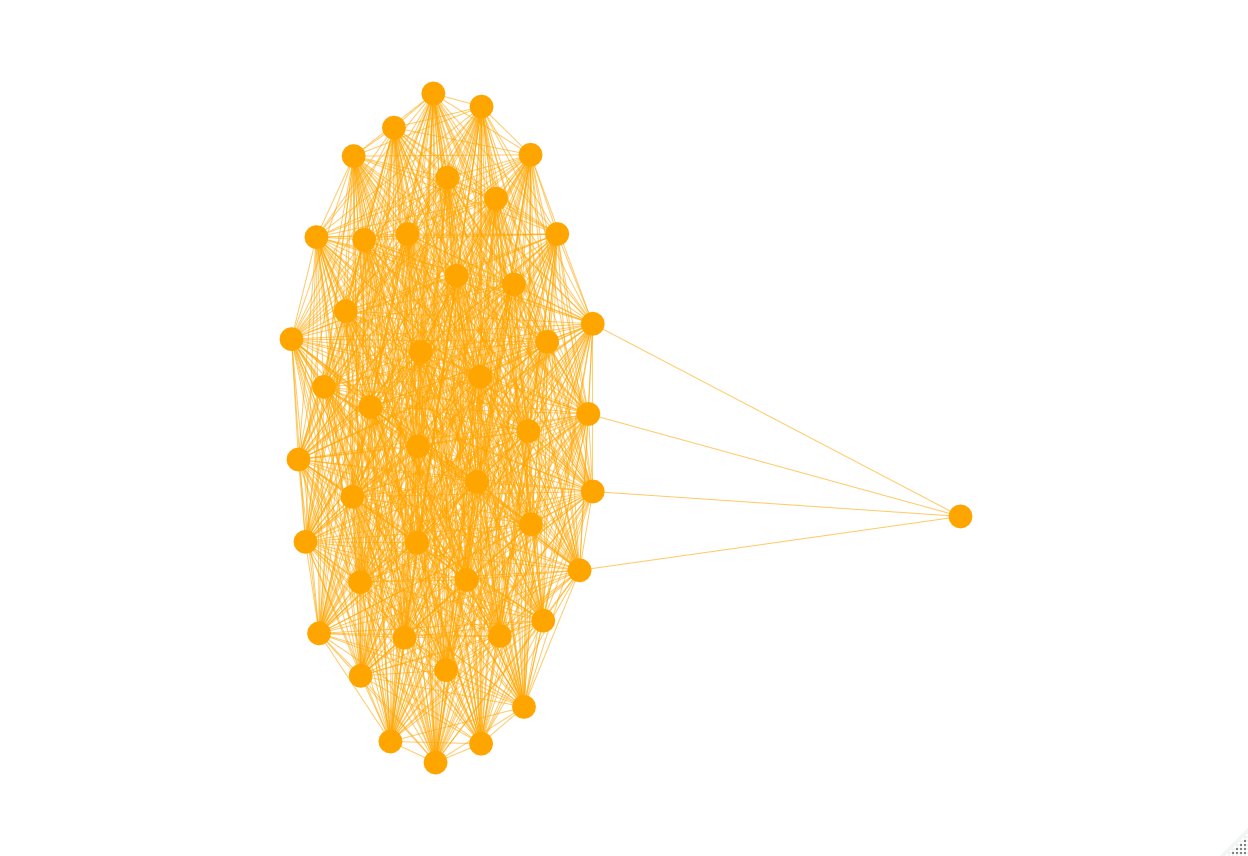
\includegraphics[scale=.15]{Reddit_Analysis/Network_Analysis/author_projection.png}}
\end{minipage}%
\begin{minipage}{.5\linewidth}
\centering
\subfloat[]{\label{birpartite:b}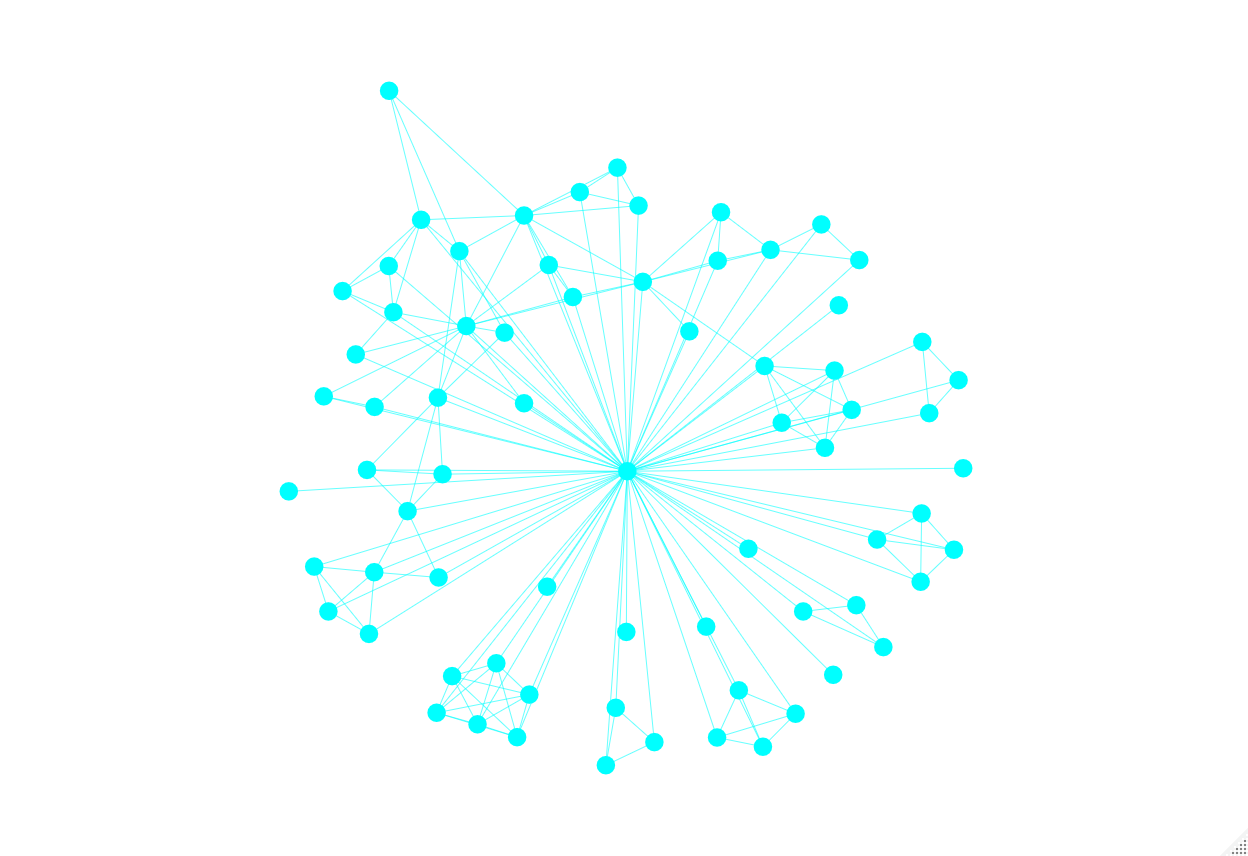
\includegraphics[scale=.15]{Reddit_Analysis/Network_Analysis/subreddit_projection.png}}
\end{minipage}\par\medskip
\centering
\subfloat[]{\label{bipartite:c}\hspace{-2em}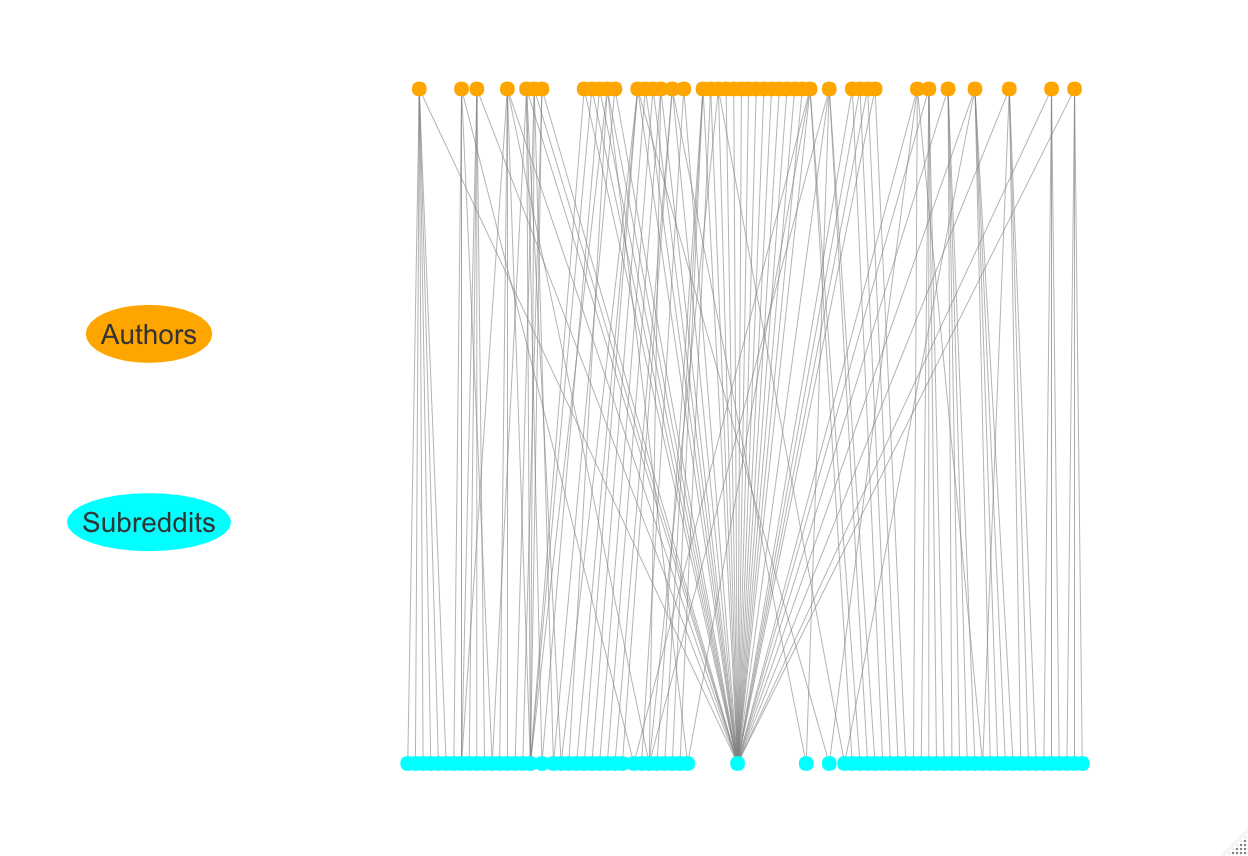
\includegraphics[scale=.25]{Reddit_Analysis/Network_Analysis/bipartite_demonstration.png}}
\caption{(a) Author projection of bipartite graph $G$. (b) Subreddit projection of bipartite graph $G$. (c) $G$ shown clearly with its bipartite structure. The central blue node in (b) and (c) is the r/CryptoCurrency subreddit.}
\label{fig:bipartite}
\end{figure}

\bibliography{references}
\end{spacing}

\end{document}
